\documentclass{article}
\usepackage{graphicx}
\usepackage{hyperref}
\usepackage[utf8]{inputenc}
\usepackage{siunitx-v2}

\graphicspath{ {./images/} }

\title{Simulazione della trasmissione simultanea di quattro segnali su un'unica linea utilizzando la tecnica FDM}
\author{Lena Giovanni Leonardo}
\date{Marzo 2022}

\begin{document}

\maketitle

\section{Scopo del progetto}
Lo scopo del progetto è la realizzazione di una simulazione software per la trasmissione di quattro segnali (due digitali
e due analogici) mediante lo stesso mezzo utilizzando la tecnica del frequency-division multiplexing (o FDM) \cite{fdm}.\\
I quattro segnali hanno la stessa frequenza e prima di essere trasmessi vengono modulati, ciascuno con una frequenza
portante diversa in modo da non avere sovrapposizioni di banda. Inoltre, tra un segnale e l'altro è prevista una
banda di guardia per evitare ulteriormente le interferenze tra un segnale e l'altro.\\
Ad ogni stadio è inoltre possibile visualizzare interattivamente ed in tempo reale i segnali, in modo da poterne comprendere
meglio il funzionamento. Viene inoltre mostrato lo spettro del segnale multiplexato, ottenuto applicando un algoritmo di
Fast Fourier Transform (FFT) \cite{fft}.\\
È infine presente un controllo che permette di rallentare il tempo per osservare meglio la generazione, modulazione e demodulazione
dei segnali. Per questioni di performance, la simulazione inizia con l'andamento del tempo rallentato di 1000 volte.

\section{Strumenti utilizzati}
La simulazione è interamente programmata nel linguaggio di programmazione Rust \cite{rust}, principalmente per le velocità che
permette di raggiungere e che non sono comparabili a nessun linguaggio di scripting interpretato come Python. La libreria
per l'interfaccia grafica si chiama egui \cite{egui}, tutti gli algoritmi per la generazione delle onde e per il filtro sono stati
implementati con gli strumenti matematici che offre il linguaggio, fatta eccezione per l'algoritmo di Fast Fourier Transform,
utilizzato per fini grafici, che viene dalla libreria rustfft \cite{rustfft}.

\section{Cenni teorici}
\subsection{Frequency-division multiplexing}
La tecnica della multiplazione a divisione di frequenza (in breve FDM) consiste nella suddivisione della banda totale disponibile
in una serie di bande più piccole e non sovrapposte tra loro, nelle quali ogni segnale può essere trasmesso indipendentemente
dagli altri e allo stesso tempo.\\
Questa tecnica si differenzia da altre tecniche come TDM che invece si basano sulla divisione del tempo, assegnando quindi
ad ogni segnale una finestra temporale ed alternando continuamente tra di esse.\\
Esempi comuni di FDM si trovano all'interno della trasmissione televisiva e radiofonica, in cui frequenze diverse vengono
trasmesse tutte allo stesso tempo. La selezione del canale, infatti, avviene sintonizzandosi su una specifica frequenza.
Ciò consente la trasmissione di una grossa quantità di dati simultaneamente, senza sprechi di banda.

\section{Generazione dei segnali}
La simulazione in tempo reale avviene con una frequenza di campionamento di \SI{2.5}{\MHz}, che corrisponde ad un periodo di
\SI{400}{\ns}. Secondo il teorema del campionamento di Nyquist-Shannon, per non perdere informazioni è sufficiente che la frequenza
di campionamento sia più il doppio della frequenza massima che si intende campionare.\\
All'interno della simulazione si raggiungono frequenze ben inferiori alla metà della frequenza di campionamento, tuttavia
per garantire una visualizzazione fluida e definita delle onde, è stata scelta una frequenza di campionamento più elevata.
Dato il periodo molto ristretto (\SI{400}{ns}), non è computazionalmente possibile eseguire l'algoritmo in tempo reale. Oltre
alla generazione dei segnali, infatti, ogni sample viene sottoposto a vari algoritmi per la visualizzazione,
modulazione e demodulazione che verranno approfonditi successivamente.\\

\begin{itemize}
    \item Onda sinusoidale a 20 kHz
    \item Onda quadra a 20 kHz
    \item Onda a dente di sega a 20 kHz
    \item Onda quadra contenente un messaggio di testo a 20 kHz
\end{itemize}

Tutti i segnali (tranne l'onda sinusoidale pura) sono generati mediante la relativa serie di Fourier con 64 iterazioni,
tuttavia questo valore può essere modificato dal codice sorgente del simulatore.

\section{Modulazione dei segnali}
Prima di poter essere trasmessi, i segnali devono essere modulati ad una specifica frequenza. Dato che si sta utilizzando la
tecnica FDM per la trasmissione dei segnali, è molto importante che le modulazioni avvengano ognuna ad una frequenza differente
dall'altra. È fondamentale calcolare la banda dei segnali modulati e fare in modo che un segnale non si sovrapponga con l'altro.
Per garantire una minore perdita durante la trasmissione, viene inoltre considerata una banda di guardia tra un segnale e
l'altro nella quale non è presente alcun segnale.\\
In alcune modulazioni (ad esempio FM), la banda teorica risultante è infinita. Secondo la regola di Carson, la banda utile nella
quale ricadono il 98\% delle frequenze è comunque limitata. Per una modulazione migliore è possibile applicare un filtro
passa banda al segnale prima che esso venga sommato con gli altri segnali.

Le modulazioni progettate per i segnali trasmessi sono riportate di seguito:

\subsection{1. Onda sinusoidale modulata in FM}
\begin{equation}
    f_m = 20 kHz
\end{equation}

\begin{equation}
    \Delta f = 75 \hspace{0.1cm} kHz
\end{equation}

\begin{equation}
    B = 2 \cdot (f_m + \Delta f) = 190 kHz
\end{equation}

\subsection{2. Onda quadra modulata in FSK}
\begin{equation}
    f_m = 20 kHz
\end{equation}

\begin{equation}
    \Delta f = 75 \hspace{0.1cm} kHz
\end{equation}

\begin{equation}
    B = 2 \cdot (\Delta f + f_m) = 190 kHz
\end{equation}

\subsection{3. Onda a dente di sega modulata in AM}
\begin{equation}
    f_m = 20 kHz
\end{equation}

\begin{equation}
    B = 2 \cdot f_m = 40 kHz
\end{equation}

\subsection{4. Onda quadra modulata in OOK}
\begin{equation}
    f_m = 20 kHz
\end{equation}

\begin{equation}
    B = 6 \cdot f_m = 120 kHz
\end{equation}

\begin{center}
    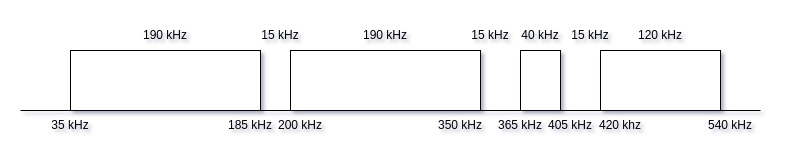
\includegraphics[width=\textwidth]{bandwidth.png}
\end{center}
Lo spettro finale, ottenuto dal calcolo delle bande e lasciando 15 kHz come bande di guardia.

\section{Multiplexing dei segnali in FDM}
Una volta che i segnali sono stati generati e modulati con delle portanti adeguatamente dimensionate, la trasmissione in FDM
avviene semplicemente sommando i quattro segnali. È possibile verificare l'efficacia di questa tecnica attraverso il grafico
dello spettro del segnale, disponibile anche nella simulazione in tempo reale. Nel caso di corretta modulazione dei segnali,
dovrebbe essere possibile visualizzare quattro gruppi di frequenze, ognuna separata dall'altra da un vuoto più o meno grande,
che rappresenta le frequenze di guardia.

\section{Separazione di ogni singolo segnale}
Per poter demodulare ed ottenere i segnali originali, è necessario isolare la banda di frequenze utili attraverso un filtro
passa-banda opportunamente dimensionato.\\
Digitalmente è possibile implementare differenti tipologie di filtri con diverse caratteristiche. Uno dei filtri che offre
le caratteristiche migliori, tra velocità di esecuzione e banda di transizione contenuta è il filtro sinc \cite{sinc},
che sfrutta l'omonima funzione, la finestra di blackman e l'operazione di convoluzione.\\

\begin{equation}
    sinc(x) = \frac{sin(x)}{x}
\end{equation}

Il filtro sinc è un filtro di tipo finite impulse response (FIR), che si differenzia dai filtri di tipo infinite impulse response
perchè il suo output si stabilizza a zero in un tempo finito. L'algoritmo per applicare un filtro sinc ad un segnale è
piuttosto semplice, richiede la convoluzione \cite{convolution} tra il segnale ed i coefficienti del filtro desiderato.\\
I coefficienti non sono altro che un vettore di numeri che rappresentano informazioni come il tipo di filtro, la banda di
transizione, la frequenza di taglio e la frequenza di campionamento. Il vettore di coefficienti si può ottenere attraverso un
tool online per il design di filtri come fiiir \cite{fiiir} oppure possono essere calcolati applicando le formule teoriche descritte
nel capitolo 16 del libro sul DSP di analog.com \cite{dsp-book-ch16}. La lunghezza dei coefficienti dipende dalla cosiddetta kernel
size. Un'elevata kernel size permette di ottenere un filtro molto preciso ma allo stesso tempo rende i calcoli più lenti.\\

\begin{center}
    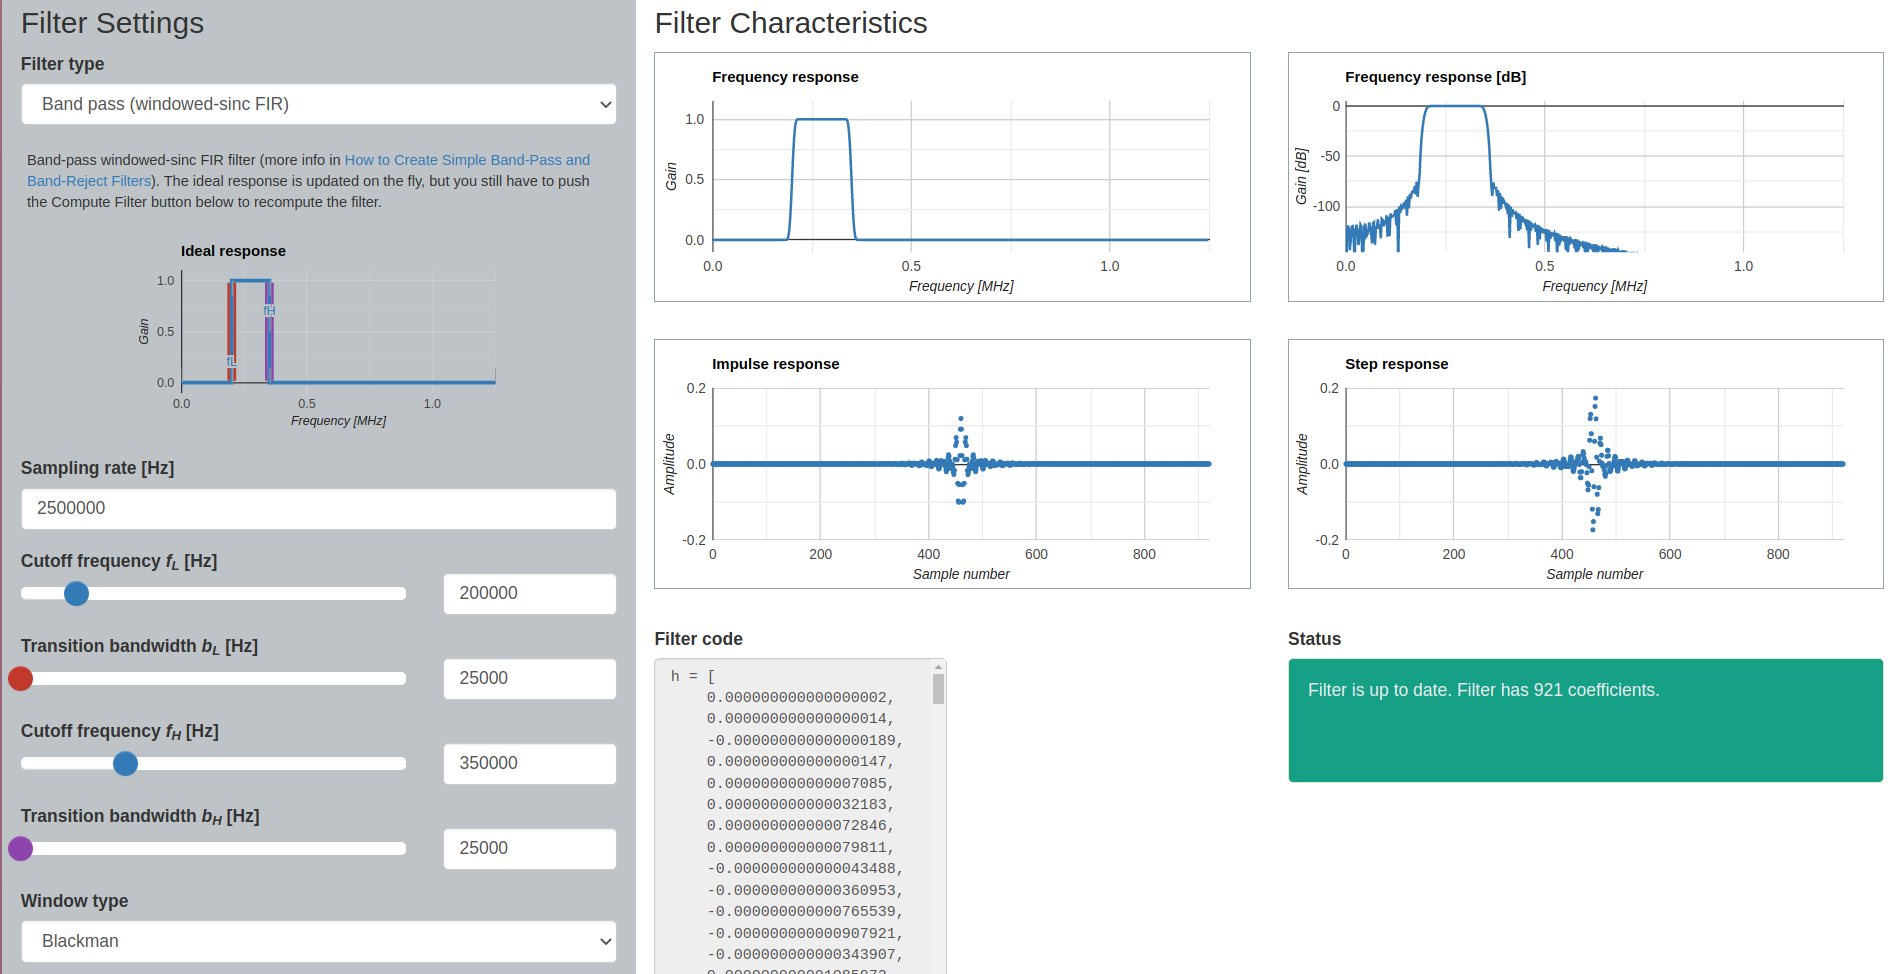
\includegraphics[width=\textwidth]{fiiir.png}
\end{center}
Progettazione di un filtro FIR con il tool disponibile su \href{https://fiiir.com}{fiiir.com}\\

\subsection{Ottimizzazione del filtro sinc ad elevate velocità}
Il collo di bottiglia in un filtro FIIIR è l'operazione di convoluzione, che ha una un fattore di complessità \cite{big_o} $O(N^2)$,
il che significa che la complessità computazionale cresce con il quadrato del numero di elementi a cui viene applicata. In un
contesto real-time, una compessità del genere non è fattibile, per questo motivo viene spesso impiegato un metodo alternativo e
più efficiente per implementare l'operazione di convoluzione. Si può infatti dimostrare che la convoluzione nel dominio del tempo
è equivalente ad una semplice moltiplicazione nel dominio della frequenza. Dato che l'algoritmo più efficiente di Fast Fourier
Transform (per trasformare il segnale nel dominio della frequenza e poi trasformarlo di nuovo nel dominio del tempo, attraverso
l'Inverse Fast Fourier Transform) ha una complessità di $O(N \cdot log (N))$, su input di elevate dimensioni questa tecnica risulta
molto più efficiente ed applicabile anche in contesti di data processing real-time.

\begin{center}
    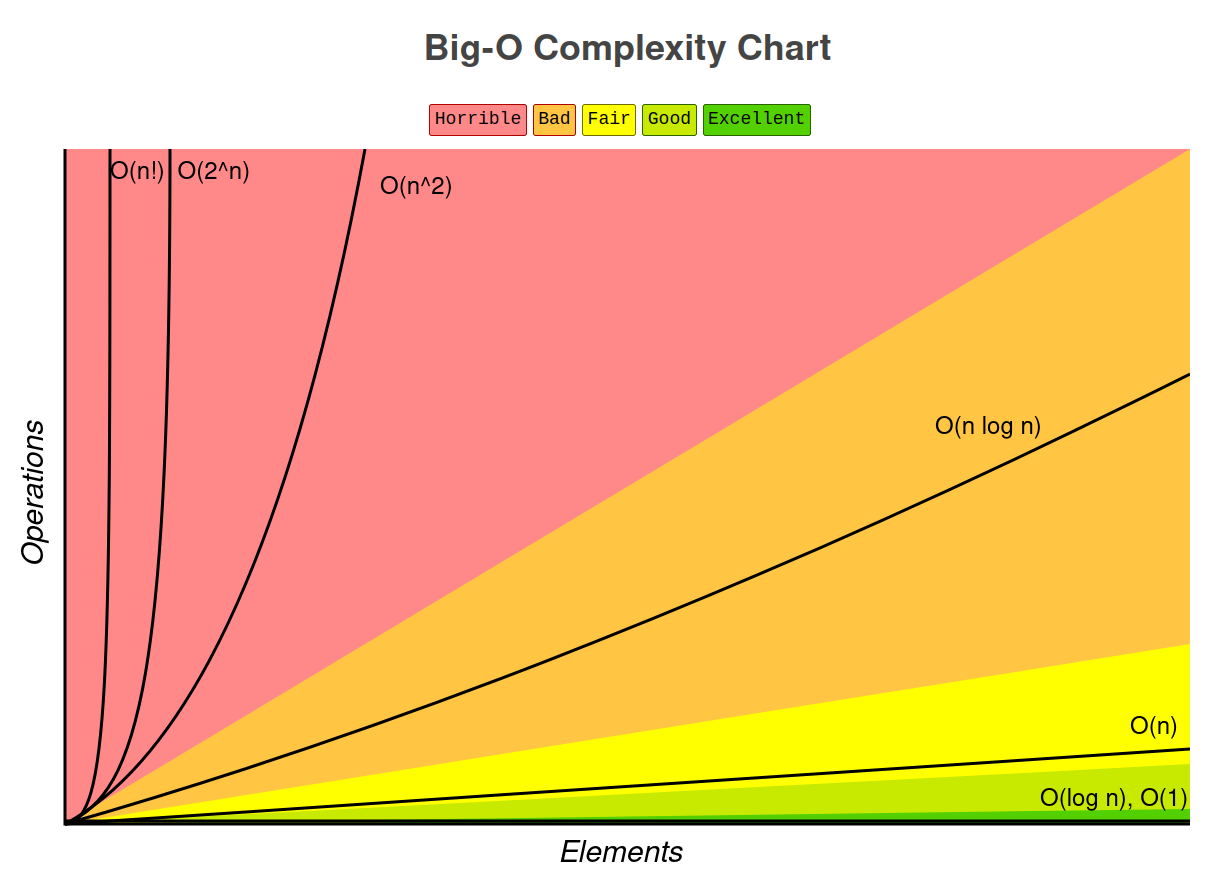
\includegraphics[width=\textwidth]{big_o.png}
\end{center}
Un grafico che mostra il concetto di Big-O notation. Come si può notare, il numero di operazioni aumenta esponenzialmente
con $O(N^2)$ mentre non ha una crescita così elevata con $O(N \cdot log (N))$.

\section{Demodulazione dei segnali}

\subsection{Demodulazione FM}
\subsection{Demodulazione FSK}
Un segnale digitale modulato in FSK è composto da un'armonica con una delle due frequenze, dette frequenze di manipolazione
($f_1$ e $f_2$) che si discostano di un fattore $\pm \Delta f$ dalla frequenza portante $f_p$ e si alternano, in base al bit
trasmesso. Ci sono vari modi per demodulare un segnale FSK all'interno di un DSP.\\
Il modo più banale è l'applicazione della trasformata di Fourier al segnale modulato, per rilevare quale delle due frequenze
di manipolazione viene trasmessa, tuttavia questo metodo è molto inefficiente (anche con le modrne implementazioni FFT) in quanto
la trasformata di Fourier rileva tutte le frequenze dello spettro, nonostante ai fini della demodulazione siano sufficienti
solo $f_1$ ed $f_2$.\\
Una tecnica molto più efficiente consiste nell'applicazione dell'algoritmo di Goertzel al segnale, che permette di rilevare
l'intensità di una singola frequenza. Applicando l'algoritmo due volte, una per $f_1$ e l'altra per $f_2$ e confrontando le due
potenze, è sufficiente determinare quella maggiore per stabilire il bit.

\subsection{Demodulazione AM}
Per la demodulazione di un segnale modulato in ampiezza è sufficiente un rivelatore d'inviluppo, implementabile attraverso un semplice
filtro passa-basso. Il fitro passa-basso utilizzato è di tipo FIR e viene implementato come il passa-banda descritto sopra.

\section{Sviluppi futuri}



\begin{thebibliography}{9}
    \bibitem{egui}
    \href{https://github.com/emilk/egui}{egui: an easy-to-use immediate mode GUI in Rust that runs on both web and native}

    \bibitem{fdm}
    \href{https://en.wikipedia.org/wiki/Frequency-division_multiplexing}{Frequency-division multiplexing}

    \bibitem{fft}
    \href{https://en.wikipedia.org/wiki/Fast_Fourier_transform}{Fast Fourier Transform}

    \bibitem{rust}
    \href{https://rust-lang.org}{Rust}

    \bibitem{rustfft}
    \href{https://docs.rs/rustfft/latest/rustfft/}{RustFFT is a high-performance FFT library written in pure Rust.}

    \bibitem{sinc}
    \href{https://en.wikipedia.org/wiki/Sinc_filter}{Sinc filter}

    \bibitem{fiiir}
    \href{https://fiiir.com/}{fiiir.com}

    \bibitem{convolution}
    \href{https://en.wikipedia.org/wiki/Convolution}{Convolution}

    \bibitem{dsp-book-ch16}
    \href{https://www.analog.com/media/en/technical-documentation/dsp-book/dsp_book_Ch16.pdf}{Dsp Book - Chapter 16}

    \bibitem{big_o}
    \href{https://en.wikipedia.org/wiki/Big_O_notation}{Big O Notation}
\end{thebibliography}


\end{document}
